%!TEX root = dissertation.tex

\chapter{Evaluación del método de evaluación (DBA) y del lenguaje para diseñar evaluaciones (SASQL)} \label{Ap:eval-metodo}

% the code below specifies where the figures are stored
\ifpdf
    \graphicspath{{Apendice/figures/PNG/}{Apendice/figures/PDF/}{Apendice/figures/}}
\else
    \graphicspath{{Apendice/figures/EPS/}{Apendice/figures/}}
\fi



\global\mdfdefinestyle{cuestionarioST}{%
linecolor=blue,linewidth=2pt,%
leftmargin=1cm,rightmargin=1cm
}

\global\mdfdefinestyle{hipotesis0}{%
linecolor=black,linewidth=1pt,%
leftmargin=1cm,rightmargin=1cm
}
Este apéndice contiene el cuestionario utilizado para la evaluación del método DBA y del lenguaje SASQL. Además, en un segundo apartado se analizan las respuestas recogidas. Las secciones de este apéndice son:

\begin{itemize}
	\item Cuestionario (ver sección~\ref{apc:eval:metodo:cuestionario})
	\item Resultados  (ver sección~\ref{apc:eval:metodo:resultados})
\end{itemize}

\newpage

\section{Cuestionario} \label{apc:eval:metodo:cuestionario}
	
	\subsection*{A. Sexo}

\begin{mdframed}[style=cuestionarioST]
			\begin{itemize}
				\item Hombre
				\item Mujer
			\end{itemize}
\end{mdframed}

	\subsection*{B. Rama}

\begin{mdframed}[style=cuestionarioST]
			\begin{itemize}
				\item Arte y humanidades
				\item Ciencias sociales y jurídicas
				\item Ciencias
				\item Ciencias de la salud
				\item Ingeniería y arquitectura
			\end{itemize}
\end{mdframed}

	
\newpage

	\subsection*{C. Cuestiones sobre el método DBA}

\begin{mdframed}[style=cuestionarioST]
	En este método, los docentes diseñan una evaluación de los estudiantes a partir de la información contenida en el registro del entorno virtual de aprendizaje y evalúan los resultados. El docente podrá aceptar y utilizar los resultados, descartarlos o redefinir una nueva evaluación para contrastar los resultados anteriores.
\end{mdframed}


	\paragraph*{C.1 ¿Considera el método DBA adecuado para obtener automáticamente indicadores de entornos de aprendizaje virtual?}

\begin{mdframed}[style=cuestionarioST]
			\begin{itemize}
				\item Sí
				\item No
				\item Ns/nc
			\end{itemize}
\end{mdframed}


	\paragraph*{C.2 ¿Cuál de las siguientes características considera que aporta el método DBA?}

Marque una opción para cada característica siendo (1) totalmente de acuerdo, (2) de acuerdo, (3) ni acuerdo ni en desacuerdo, (4) en desacuerdo y (5) totalmente en desacuerdo.

\begin{table}[H]
  \begin{center}
  \begin{tabular}{| m{5cm} | c | c | c | c | c |}
    \hline
    CARACTERISTICAS & (1) & (2) & (3) & (4) & (5) \\
    \hline
    \hline
    Objetividad &  &  & & & \\
    \hline
    Adaptabilidad &  &  & & & \\
    \hline
    Sistematicidad &  &  & & &  \\
    \hline
    Flexibilidad &  &  & & &  \\
    \hline
    Fiabilidad &  &  & & &  \\
    \hline
  \end{tabular}
\end{center}
\caption{Selección de características del método DBA}
\label{tab:ap:caracteristicas:metodo}
\end{table}

\newpage

\subsection*{D. Cuestiones sobre el lenguaje SASQL}

\begin{mdframed}[style=cuestionarioST]
	Con este lenguaje los docentes pueden diseñar evaluaciones a partir de la información contenida en el registro de aprendizaje virtual. 
\end{mdframed}

	\paragraph*{D.1 ¿Considera que el lenguaje presentado es útil para diseñar y contrastar estrategias de evaluación a partir de los registros de actividad de los entornos de aprendizaje virtual?}

\begin{mdframed}[style=cuestionarioST]
			\begin{itemize}
				\item Sí
				\item No
				\item Ns/Nc
			\end{itemize}
\end{mdframed}


	\paragraph*{D.2 ¿Cuáles de las siguientes características considera que aporta el lenguaje presentado?}

Marque una opción para cada característica siendo (1) totalmente de acuerdo, (2) de acuerdo, (3) ni acuerdo ni en desacuerdo, (4) en desacuerdo y (5) totalmente en desacuerdo.

\begin{table}[H]
  \begin{center}
  \begin{tabular}{| m{5cm} | c | c | c | c | c |}
    \hline
    CARACTERISTICAS & (1) & (2) & (3) & (4) & (5) \\
    \hline
    \hline
    Facilidad de aprendizaje &  &  & & & \\
    \hline
    Eficacia &  &  & & & \\
    \hline
    Ahorra tiempo &  & & & &  \\
    \hline
    Escalabilidad &  & & & &  \\
    \hline
    Capacidad de reutilización &  &  & & &  \\
    \hline
    Fiabilidad &  &  & & & \\
    \hline
  \end{tabular}
\end{center}
\caption{Selección de características del lenguaje SASQL}
\label{tab:ap:caracteristicas:sasql}
\end{table}

\newpage

	\paragraph*{D.3 Tomando como ejemplo la siguiente consulta del DSL, utilizada para obtener información de la interacción de los estudiantes en el foro del campus virtual:}

\begin{minted}[linenos,frame=lines,
               framesep=2mm]{pascal}
Evidence interaccion_foro:  
	get students 
	show interaction 
	in forum.
\end{minted}


\begin{mdframed}[style=cuestionarioST]
	¿Considera entendible la consultas del DSL?
			\begin{itemize}
				\item Sí
				\item No
				\item Ns/Nc
			\end{itemize}
\end{mdframed}


	\paragraph*{D.4 Tomando como ejemplo los resultados que se obtienen de la consulta anterior:}

\begin{figure}[H]
  \begin{center}
    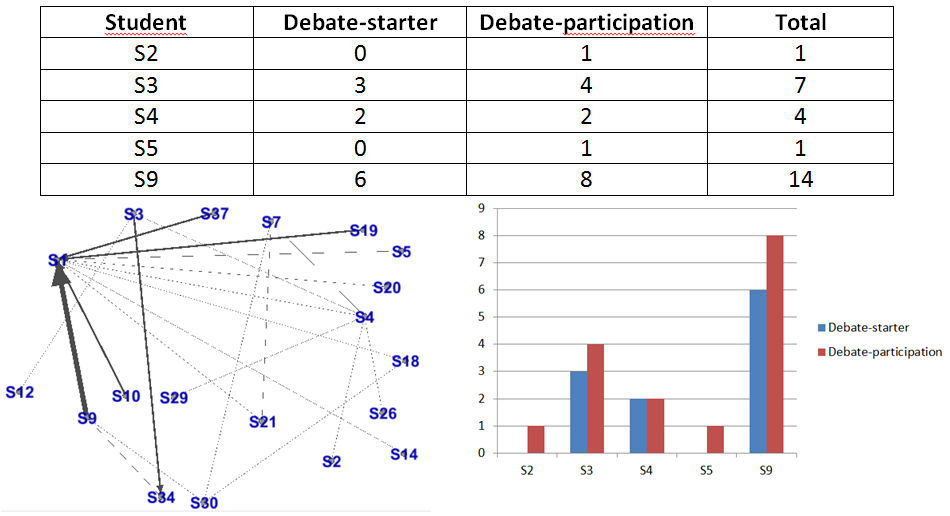
\includegraphics[scale=0.4]{ResultadosConsulta.png}
  \end{center}
  \caption{Resultados consulta}
  \label{fig:ape:resultados:consulta}
\end{figure}

\begin{mdframed}[style=cuestionarioST]
	¿Considera los resultados entendibles?
			\begin{itemize}
				\item Sí
				\item No
				\item Ns/Nc
			\end{itemize}
\end{mdframed}



\newpage

% RESULTADOS COPIADOS DEL OTRO.
\section{Resultados} \label{apc:eval:metodo:resultados}

En esta sección se muestran y analizan en detalle los resultados del cuestionario. %Los comentarios sobre los resultados de los profesores se muestran en el capítulo X (esto se dice en la tesis de la uoc, tendré que ver qué comento yo).

\subsection{Participantes}

En este cuestionario participaron docentes que asistieron a las Jornadas de Innovación Docente de la Universidad de Cádiz. Se realizó una presentación del método y la herramienta, y tras un turno de preguntas, se pasó el cuestionario mostrado en el apartado anterior.

En total fueron completados 31 cuestionarios, distribuidos tal y cómo se resume en la tabla~\ref{tab:evalmetodo:encuesta:rama:sexo}.

\begin{table}[H]
  \begin{center}
  \begin{tabular}{| l | r | r | r | r |}
    \hline
    Rama \ Sexo & Hombre & Mujer & Ns/Nc & Total \\
    \hline
    \hline
    Arte y humanidades & 1 & 4 & 0 & 5  \\
    \hline
    Ciencias & 3 & 2 & 0 & 5  \\
    \hline
    Ciencias de la salud & 6 & 0 & 0 & 6  \\
    \hline
    Ciencias sociales y jurídicas & 2 & 2 & 1 & 5  \\
    \hline
    Ingeniería y arquitectura & 6 & 4 & 0 & 10 \\
    \hline
  \end{tabular}
\end{center}
\caption{Resumen de distribución de participantes por rama y sexo}
\label{tab:evalmetodo:encuesta:rama:sexo}
\end{table}

Para afinar en la independencia de las respuestas dadas por los docentes se agruparon sus ramas con respecto a las ramas principales del conocimiento:

\begin{itemize}
\item \emph{EHSE, Earth \& Health Sciences and Engineering}: Ciencias, Ciencias de la salud e Ingeniería y arquitectura.
\item \emph{SSH, Social Sciences and Humanities}: Arte y humanidades y Ciencias sociales y jurídicas.
\end{itemize}

%-----------------------------------------------------------------
%-----------------------------------------------------------------
%-----------------------------------------------------------------
\subsection{Evaluación del método DBA}

Con respecto a la pregunta sobre la idoneidad del método DBA, el resumen de las respuestas puede verse en la tabla~\ref{tab:evalmetodo:encuesta:metodoDBA:rama}.

\begin{table}[H]
  \begin{center}
  \begin{tabular}{| l | l | r | r | r |}
    \hline
    & Rama & Sí & No & Total \\
    \hline
    \hline
    \multirow{2}{2.5cm}{SSH} & Arte y humanidades & 4 & 1 & 5  \\
    \cline{2-5}
    & Ciencias sociales y jurídicas & 3 & 2 & 5  \\
    \hline
    \multirow{3}{2.5cm}{EHSE} & Ciencias & 5 & 0 & 5  \\
    \cline{2-5}
    & Ciencias de la salud & 5 & 1 & 6  \\
    \cline{2-5}
    & Ingeniería y arquitectura & 9 & 1 & 10 \\
    \hline
  \end{tabular}
\end{center}
\caption{Consideración de idoneidad del método DBA por ramas}
\label{tab:evalmetodo:encuesta:metodoDBA:rama}
\end{table}

Un 84\percentage{ }de los encuestados (26 de 31) consideraron el método DBA adecuado. Para dar validez a los resultados es necesario determinar la independencia de los mismos.

En primer lugar, para determinar si existe relación entre la respuesta de cada docente y su rama se define la siguiente hipótesis nula:

\medskip
\begin{mdframed}[style=hipotesis0]
$H_0$: \emph{La consideración por parte de un docente de que el método DBA sea o no válido es independiente de la rama de dicho docente}
\end{mdframed}

\medskip
Para contrastar la hipótesis se utilizó el test exacto de Fisher, no pudiéndose rechazar la hipótesis con un \textbf{p-valor de 0,6142}, superior al umbral de significación del 0,005. Por lo que se concluye que, con una significación del 5\percentage, los datos son independientes.

En segundo lugar, para determinar si existe relación entre la respuesta de cada docente y su rama principal se define la siguiente hipótesis nula:

\medskip
\begin{mdframed}[style=hipotesis0]
$H_0$: \emph{La consideración por parte de un docente de que el método DBA sea o no válido es independiente de si dicho docente es de EHSE o de SSH}
\end{mdframed}

\medskip
Para contrastar la hipótesis se utilizó el test exacto de Fisher, no pudiéndose rechazar la hipótesis con un \textbf{p-valor de 0,2955}, superior al umbral de significación del 0,005. Por lo que se concluye que, con una significación del 5\percentage, los datos son independientes.


\subsubsection{Características del método DBA}

A continuación se preguntó a los encuestados sobre su consideración acerca de en qué medida el método DBA satisface cada una de las características que se esperan del mismo. Estas características son \emph{objetividad}, \emph{adaptabilidad}, \emph{sistematicidad}, \emph{flexibilidad} y \emph{fiabilidad}. Para su evaluación se preguntó sobre ellos en una escala Likert de cinco puntos: totalmente de acuerdo, de acuerdo, ni de acuerdo ni en desacuerdo, en desacuerdo y totalmente en desacuerdo. 

En la tabla~\ref{tab:evalmetodo:encuesta:metodoDBA:caracteristicas} puede verse el resumen de las respuestas dadas.

\begin{table}[H]
  \begin{center}
  \begin{tabular}{| l | r | r | r | r | r |}
    \hline
    \multirow{3}{1.9cm}{Características} & \multirow{3}{1.9cm}{\centering Totalmente de acuerdo} & \multirow{3}{1.2cm}{\centering De acuerdo} & \multirow{3}{2.3cm}{\centering Ni de acuerdo ni en desacuerdo} & \multirow{3}{1.8cm}{\centering En desacuerdo} & \multirow{3}{1.9cm}{\centering Totalmente en desacuerdo} \\
    & & & & & \\
    & & & & & \\
    \hline
    \hline
    Objetividad & 23\percentage & 23\percentage & 32\percentage & 19\percentage & 3\percentage \\
    \hline
    Adaptabilidad & 16\percentage & 45\percentage & 23\percentage & 13\percentage & 3\percentage \\
    \hline
    Sistematicidad & 40\percentage & 30\percentage & 20\percentage & 10\percentage & 0\percentage \\
    \hline
    Flexibilidad & 19\percentage & 42\percentage & 26\percentage & 13\percentage & 0\percentage \\
    \hline
    Fiabilidad & 6\percentage & 39\percentage & 26\percentage & 23\percentage & 6\percentage \\
    \hline
  \end{tabular}
\end{center}
\caption{Evaluación de las características del método DBA}
\label{tab:evalmetodo:encuesta:metodoDBA:caracteristicas}
\end{table}

En general los docentes muestran su conformidad para las características. En primer lugar, para la adaptabilidad, la sistematicidad y la flexibilidad, el nivel de aceptación de los docentes para el método está entre el 61 y el 70\percentage. En segundo lugar, para las características de la fiabilidad y la objetividad la suma de las dos primeras opciones está en torno al 45\percentage.

\newpage
\paragraph*{Objetividad}

El resumen de respuestas para la característica de la objetividad puede verse en las figuras~\ref{fig:evalmetodo:dba:objetividad} y~\ref{fig:evalmetodo:dba:objetividad:rama}.

\begin{figure}[h]
  \begin{center}
    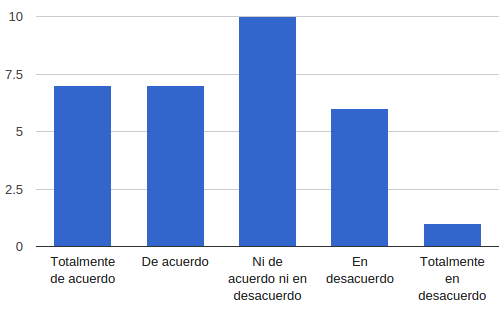
\includegraphics[scale=0.5]{C_DBA_objetividad.png}
  \end{center}
  \caption{Resumen de votos para la característica de la objetividad}
  \label{fig:evalmetodo:dba:objetividad}
\end{figure}

Hay una mayoría de docentes que están en mayor o menor medida de acuerdo con la consecución de esta característica (14 de 31). Además, 10 docentes mostraron una posición neutral con respecto a esta característica, mientras que 7 estuvieron en desacuerdo. Los datos no son significativos en lo que respecta a la rama de cada docente.

\begin{figure}[h]
  \begin{center}
    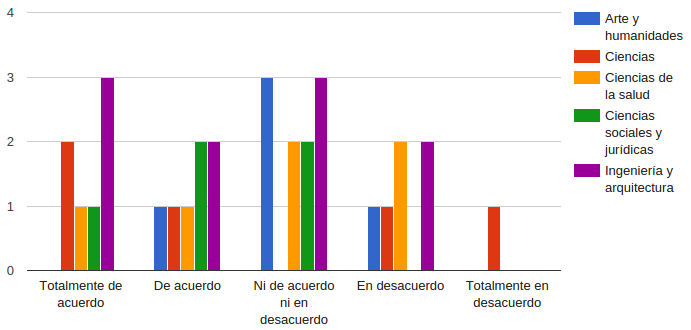
\includegraphics[scale=0.5]{C_DBA_objetividad_rama.png}
  \end{center}
  \caption{Resumen de votos para la característica de la objetividad por rama}
  \label{fig:evalmetodo:dba:objetividad:rama}
\end{figure}

\newpage
\paragraph*{Adaptabilidad}

El resumen de respuestas para la característica de la adaptabilidad puede verse en las figuras~\ref{fig:evalmetodo:dba:adaptabilidad} y~\ref{fig:evalmetodo:dba:adaptabilidad:rama}.

\begin{figure}[h]
  \begin{center}
    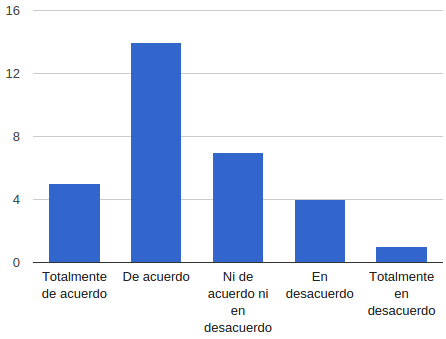
\includegraphics[scale=0.5]{C_DBA_adaptabilidad.png}
  \end{center}
  \caption{Resumen de votos para la característica de la adaptabilidad}
  \label{fig:evalmetodo:dba:adaptabilidad}
\end{figure}

Hay una mayoría de docentes que están en mayor o menor medida de acuerdo con la consecución de esta característica (19 de 31). Además, 7 docentes mostraron una posición neutral con respecto a esta característica, mientras que 5 estuvieron en desacuerdo. Cabe destacar que los docentes que estuvieron en desacuerdo fueron docentes de Ciencias o Ciencias de la salud.

\begin{figure}[h]
  \begin{center}
    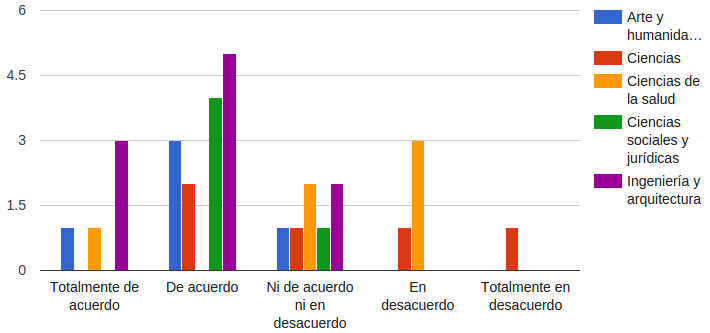
\includegraphics[scale=0.5]{C_DBA_adaptabilidad_rama.png}
  \end{center}
  \caption{Resumen de votos para la característica de la adaptabilidad por rama}
  \label{fig:evalmetodo:dba:adaptabilidad:rama}
\end{figure}

\newpage
\paragraph*{Sistematicidad}

El resumen de respuestas para la característica de la sistematicidad puede verse en las figuras~\ref{fig:evalmetodo:dba:sistematicidad} y~\ref{fig:evalmetodo:dba:sistematicidad:rama}.

\begin{figure}[h]
  \begin{center}
    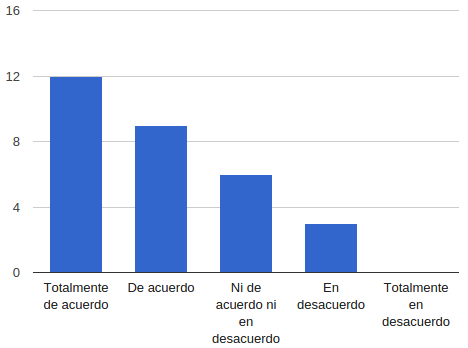
\includegraphics[scale=0.5]{C_DBA_sistematicidad.png}
  \end{center}
  \caption{Resumen de votos para la característica de la sistematicidad}
  \label{fig:evalmetodo:dba:sistematicidad}
\end{figure}

Hay una mayoría de docentes que están en mayor o menor medida de acuerdo con la consecución de esta característica (21 de 31). Además, 6 docentes mostraron una posición neutral con respecto a esta característica, mientras que 3 estuvieron en desacuerdo. Cabe destacar que los docentes que estuvieron en desacuerdo fueron docentes de Ciencias o Ciencias de la salud, mientras que todos los de Ingeniería y arquitectura están en los votos de conformidad.

\begin{figure}[h]
  \begin{center}
    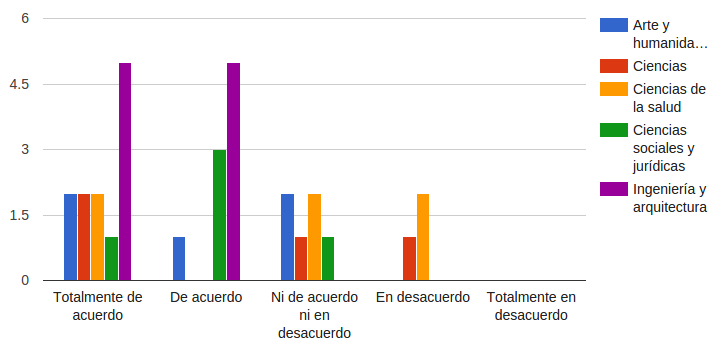
\includegraphics[scale=0.5]{C_DBA_sistematicidad_rama.png}
  \end{center}
  \caption{Resumen de votos para la característica de la sistematicidad por rama}
  \label{fig:evalmetodo:dba:sistematicidad:rama}
\end{figure}


\newpage
\paragraph*{Flexibilidad}

El resumen de respuestas para la característica de la flexibilidad puede verse en las figuras~\ref{fig:evalmetodo:dba:flexibilidad} y~\ref{fig:evalmetodo:dba:flexibilidad:rama}.

\begin{figure}[h]
  \begin{center}
    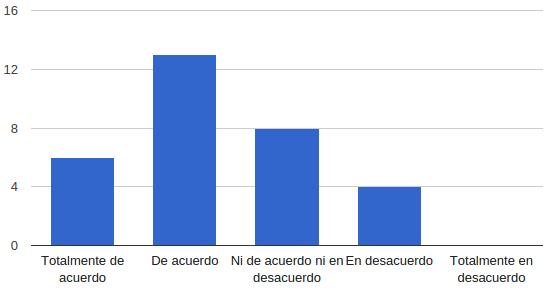
\includegraphics[scale=0.5]{C_DBA_flexibilidad.png}
  \end{center}
  \caption{Resumen de votos para la característica de la flexibilidad}
  \label{fig:evalmetodo:dba:flexibilidad}
\end{figure}

Hay una mayoría de docentes que están en mayor o menor medida de acuerdo con la consecución de esta característica (19 de 31). Además, 8 docentes mostraron una posición neutral con respecto a esta característica, mientras que 4 estuvieron en desacuerdo. También los docentes que estuvieron en desacuerdo fueron docentes de Ciencias o Ciencias de la salud.

\begin{figure}[h]
  \begin{center}
    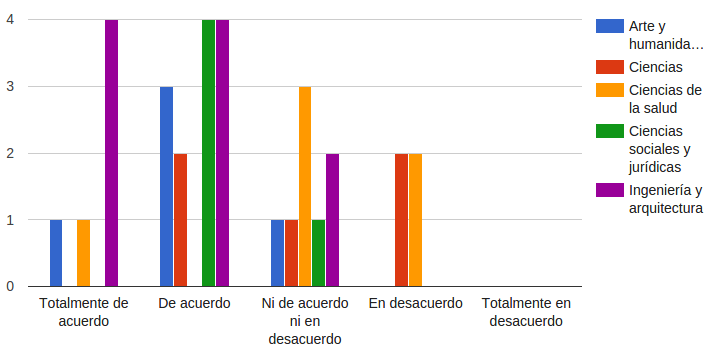
\includegraphics[scale=0.5]{C_DBA_flexibilidad_rama.png}
  \end{center}
  \caption{Resumen de votos para la característica de la flexibilidad por rama}
  \label{fig:evalmetodo:dba:flexibilidad:rama}
\end{figure}


\newpage
\paragraph*{Fiabilidad}

El resumen de respuestas para la característica de la fiabilidad puede verse en las figuras~\ref{fig:evalmetodo:dba:fiabilidad} y~\ref{fig:evalmetodo:dba:fiabilidad:rama}.

\begin{figure}[h]
  \begin{center}
    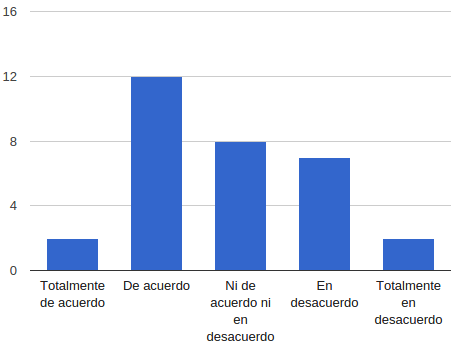
\includegraphics[scale=0.5]{C_DBA_fiabilidad.png}
  \end{center}
  \caption{Resumen de votos para la característica de la fiabilidad}
  \label{fig:evalmetodo:dba:fiabilidad}
\end{figure}

Hay una mayoría de docentes que están en mayor o menor medida de acuerdo con la consecución de esta característica (14 de 31). Además, 8 docentes mostraron una posición neutral con respecto a esta característica, mientras que 9 estuvieron en desacuerdo. Los datos no son significativos en lo que respecta a la rama de cada docente.

\begin{figure}[h]
  \begin{center}
    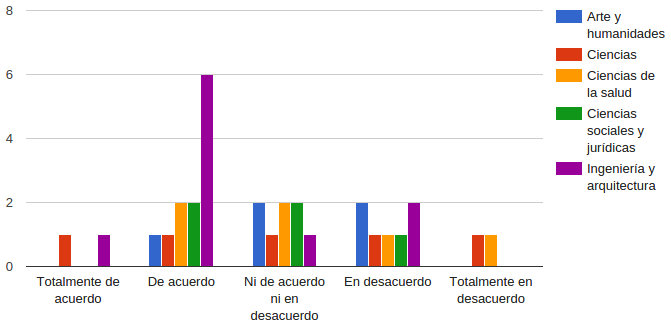
\includegraphics[scale=0.5]{C_DBA_fiabilidad_rama.png}
  \end{center}
  \caption{Resumen de votos para la característica de la fiabilidad por rama}
  \label{fig:evalmetodo:dba:fiabilidad:rama}
\end{figure}


%-----------------------------------------------------------------
%-----------------------------------------------------------------
%-----------------------------------------------------------------
\subsection{Evaluación del DSL}

Con respecto a la pregunta sobre la idoneidad del DSL, el resumen de las respuestas puede verse en la tabla~\ref{tab:evalmetodo:encuesta:DSL:rama}.

\begin{table}[H]
  \begin{center}
  \begin{tabular}{| l | l | r | r | r |}
    \hline
    & Rama & Sí & No & Total \\
    \hline
    \hline
    \multirow{2}{2.5cm}{SSH} & Arte y humanidades & 4 & 1 & 5  \\
    \cline{2-5}
    & Ciencias sociales y jurídicas & 3 & 2 & 5  \\
    \hline
    \multirow{3}{2.5cm}{EHSE} & Ciencias & 5 & 0 & 5  \\
    \cline{2-5}
    & Ciencias de la salud & 5 & 1 & 6  \\
    \cline{2-5}
    & Ingeniería y arquitectura & 9 & 1 & 10 \\
    \hline
  \end{tabular}
\end{center}
\caption{Consideración de idoneidad del DSL por ramas}
\label{tab:evalmetodo:encuesta:DSL:rama}
\end{table}

Un 84\percentage{ }de los encuestados (26 de 31) consideraron el DSL adecuado. Para dar validez a los resultados es necesario determinar la independencia de los mismos.

En primer lugar, para determinar si existe relación entre la respuesta de cada docente y su rama se define la siguiente hipótesis nula:

\medskip
\begin{mdframed}[style=hipotesis0]
$H_0$: \emph{La consideración por parte de un docente de que el DSL sea o no válido es independiente de la rama de dicho docente}
\end{mdframed}

\medskip
Para contrastar la hipótesis se utilizó el test exacto de Fisher, no pudiéndose rechazar la hipótesis con un \textbf{p-valor de 0,6142}, superior al umbral de significación del 0,005. Por lo que se concluye que, con una significación del 5\percentage, los datos son independientes.

En segundo lugar, para determinar si existe relación entre la respuesta de cada docente y su rama principal se define la siguiente hipótesis nula:

\medskip
\begin{mdframed}[style=hipotesis0]
$H_0$: \emph{La consideración por parte de un docente de que el DSL sea o no válido es independiente de si  dicho docente es de EHSE o de SSH}
\end{mdframed}

\medskip
Para contrastar la hipótesis se utilizó el test exacto de Fisher, no pudiéndose rechazar la hipótesis con un \textbf{p-valor de 0,2955}, superior al umbral de significación del 0,005. Por lo que se concluye que, con una significación del 5\percentage, los datos son independientes.

\subsubsection{Características del DSL}

A continuación se preguntó a los encuestados sobre su consideración acerca de en qué medida el DSL satisface cada una de las características que se esperan del mismo. Estas características son \emph{facilidad de aprendizaje}, \emph{eficacia}, \emph{ahorra tiempo}, \emph{escalabilidad}, \emph{capacidad de reutilización} y \emph{fiabilidad}. Para su evaluación se preguntó sobre ellos en una escala Likert de cinco puntos: totalmente de acuerdo, de acuerdo, ni de acuerdo ni en desacuerdo, en desacuerdo y totalmente en desacuerdo. 

En la tabla~\ref{tab:evalmetodo:encuesta:DSL:caracteristicas} puede verse el resumen de las respuestas dadas.

\begin{table}[H]
  \begin{center}
  \begin{tabular}{| m{2.5cm} | r | r | r | r | r |}
    \hline
    \multirow{3}{2.5cm}{Características} & \multirow{3}{1.9cm}{\centering Totalmente de acuerdo} & \multirow{3}{1.2cm}{\centering De acuerdo} & \multirow{3}{2.3cm}{\centering Ni de acuerdo ni en desacuerdo} & \multirow{3}{1.8cm}{\centering En desacuerdo} & \multirow{3}{1.9cm}{\centering Totalmente en desacuerdo} \\
    & & & & & \\
    & & & & & \\
    \hline
    \hline
    Facilidad de aprendizaje & 19\percentage & 32\percentage & 39\percentage & 7\percentage & 3\percentage \\
    \hline
    Eficacia & 13\percentage & 45\percentage & 26\percentage & 16\percentage & 0\percentage \\
    \hline
    Ahorra tiempo & 32\percentage & 23\percentage & 32\percentage & 13\percentage & 0\percentage \\
    \hline
    Escalabilidad & 23\percentage & 23\percentage & 35\percentage & 19\percentage & 0\percentage \\
    \hline
    Capacidad de reutilización & 26\percentage & 32\percentage & 29\percentage & 6,5\percentage & 6,5\percentage \\
    \hline
    Fiabilidad & 6\percentage & 29\percentage & 42\percentage & 23\percentage & 0\percentage \\
    \hline
  \end{tabular}
\end{center}
\caption{Evaluación de las características del DSL}
\label{tab:evalmetodo:encuesta:DSL:caracteristicas}
\end{table}

Puede decirse que el rechazo al hecho de que el DSL proporcione dichas características es bajo, pues para todas las características es inferior al 20\percentage{ }(excepto para la fiablidad que es el 23\percentage.

Sin embargo, es un hecho que el nivel de aceptación (sumando los de acuerdo con los totalmente de acuerdo) es levemente superior al 50\percentage, habiendo también un grupo nutrido de docentes que se sitúan en el punto neutro.

\newpage
\paragraph*{Facilidad de aprendizaje}

El resumen de respuestas para la característica de la facilidad de aprendizaje del DSL puede verse en las figuras~\ref{fig:evalmetodo:dsl:aprendizaje} y~\ref{fig:evalmetodo:dsl:aprendizaje:rama}.

\begin{figure}[h]
  \begin{center}
    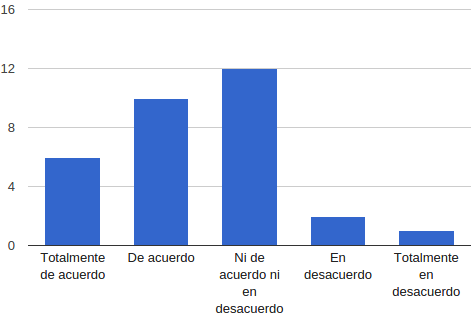
\includegraphics[scale=0.5]{C_DSL_aprendizaje.png}
  \end{center}
  \caption{Resumen de votos para la característica de la facilidad de aprendizaje}
  \label{fig:evalmetodo:dsl:aprendizaje}
\end{figure}

Hay una mayoría de docentes que están en mayor o menor medida de acuerdo con la consecución de esta característica (16 de 31). Además, 12 docentes mostraron una posición neutral con respecto a esta característica, mientras que 3 estuvieron en desacuerdo. Los docentes que estuvieron en desacuerdo fueron nuevamente docentes de Ciencias o Ciencias de la salud.

\begin{figure}[h]
  \begin{center}
    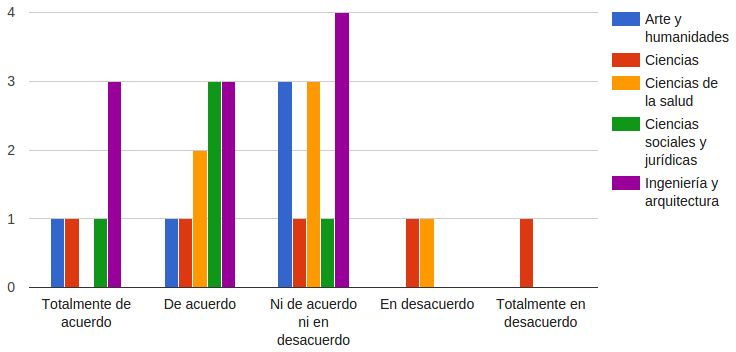
\includegraphics[scale=0.5]{C_DSL_aprendizaje_rama.png}
  \end{center}
  \caption{Resumen de votos para la característica de la facilidad de aprendizaje por rama}
  \label{fig:evalmetodo:dsl:aprendizaje:rama}
\end{figure}

\newpage
\paragraph*{Eficacia}

El resumen de respuestas para la característica de la eficacia del DSL puede verse en las figuras~\ref{fig:evalmetodo:dsl:eficacia} y~\ref{fig:evalmetodo:dsl:eficacia:rama}.

\begin{figure}[h]
  \begin{center}
    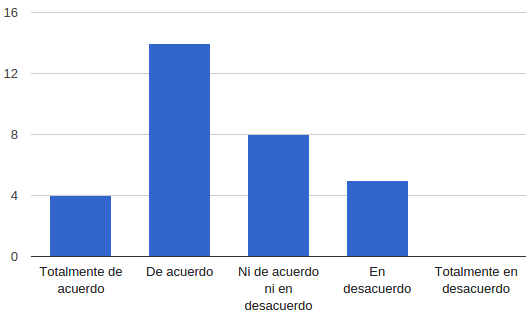
\includegraphics[scale=0.5]{C_DSL_eficacia.png}
  \end{center}
  \caption{Resumen de votos para la característica de la eficacia}
  \label{fig:evalmetodo:dsl:eficacia}
\end{figure}

Hay una mayoría de docentes que están en mayor o menor medida de acuerdo con la consecución de esta característica (18 de 31). Además, 8 docentes mostraron una posición neutral con respecto a esta característica, mientras que 5 estuvieron en desacuerdo. %Cabe destacar que los docentes que estuvieron en desacuerdo fueron docentes de la rama principal de las \emph{EHSE}.

\begin{figure}[h]
  \begin{center}
    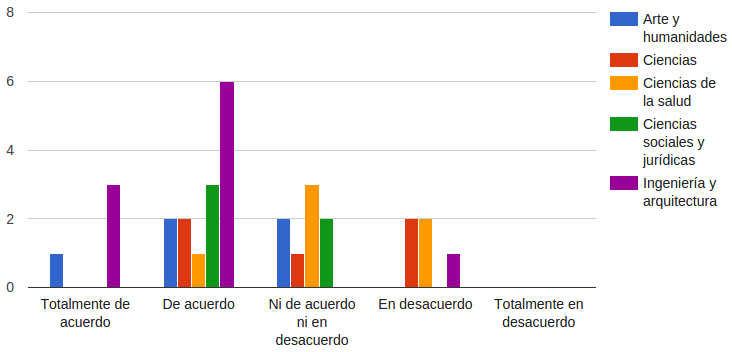
\includegraphics[scale=0.5]{C_DSL_eficacia_rama.png}
  \end{center}
  \caption{Resumen de votos para la característica de la eficacia por rama}
  \label{fig:evalmetodo:dsl:eficacia:rama}
\end{figure}

\newpage
\paragraph*{Ahorra tiempo}

El resumen de respuestas para la característica del ahorro del tiempo del DSL puede verse en las figuras~\ref{fig:evalmetodo:dsl:ahorro} y~\ref{fig:evalmetodo:dsl:ahorro:rama}.

\begin{figure}[h]
  \begin{center}
    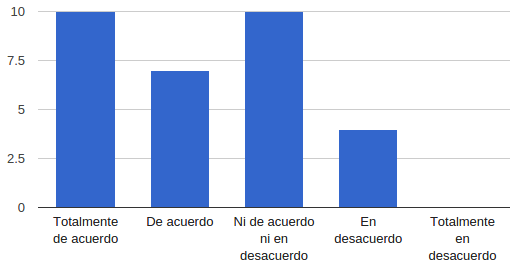
\includegraphics[scale=0.5]{C_DSL_ahorro.png}
  \end{center}
  \caption{Resumen de votos para la característica del ahorro del timepo}
  \label{fig:evalmetodo:dsl:ahorro}
\end{figure}

Hay una mayoría de docentes que están en mayor o menor medida de acuerdo con la consecución de esta característica (17 de 31). Además, 10 docentes mostraron una posición neutral con respecto a esta característica, mientras que 4 estuvieron en desacuerdo.

\begin{figure}[h]
  \begin{center}
    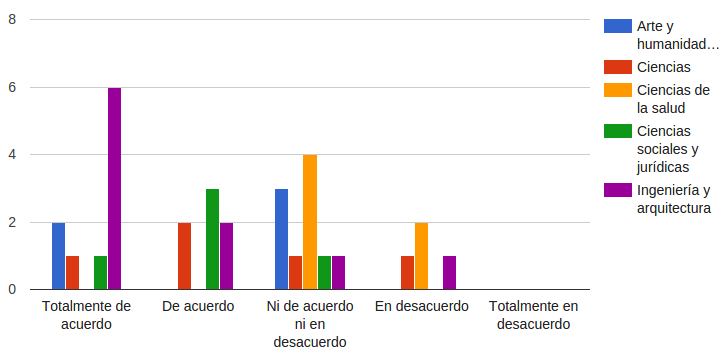
\includegraphics[scale=0.5]{C_DSL_ahorro_rama.png}
  \end{center}
  \caption{Resumen de votos para la característica del ahorro del tiempo}
  \label{fig:evalmetodo:dsl:ahorro:rama}
\end{figure}

\newpage
\paragraph*{Escalabilidad}

El resumen de respuestas para la característica de la escalabilidad del DSL puede verse en las figuras~\ref{fig:evalmetodo:dsl:escalabilidad} y~\ref{fig:evalmetodo:dsl:escalabilidad:rama}.

\begin{figure}[h]
  \begin{center}
    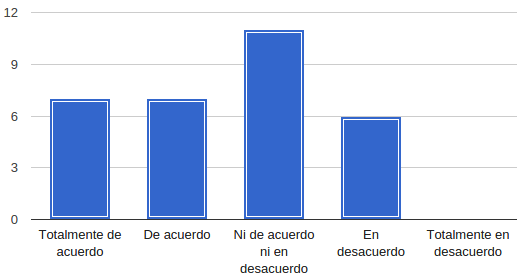
\includegraphics[scale=0.5]{C_DSL_escalabilidad.png}
  \end{center}
  \caption{Resumen de votos para la característica de la escalabilidad}
  \label{fig:evalmetodo:dsl:escalabilidad}
\end{figure}

Hay una mayoría de docentes que están en mayor o menor medida de acuerdo con la consecución de esta característica (14 de 31). Además, 10 docentes mostraron una posición neutral con respecto a esta característica, mientras que 6 estuvieron en desacuerdo.

\begin{figure}[h]
  \begin{center}
    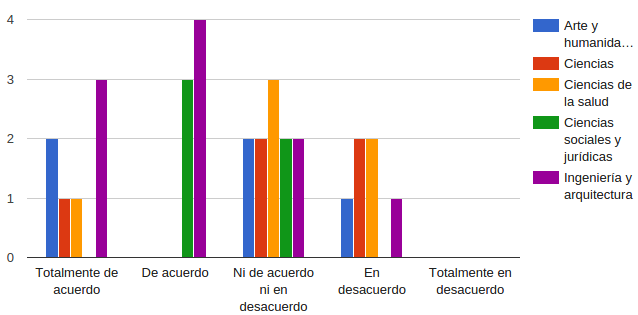
\includegraphics[scale=0.5]{C_DSL_escalabilidad_rama.png}
  \end{center}
  \caption{Resumen de votos para la característica de la escalabilidad por rama}
  \label{fig:evalmetodo:dsl:escalabilidad:rama}
\end{figure}

\newpage
\paragraph*{Capacidad de reutilización}

El resumen de respuestas para la característica de la capacidad de reutilización del DSL puede verse en las figuras~\ref{fig:evalmetodo:dsl:reutilizable} y~\ref{fig:evalmetodo:dsl:reutilizable:rama}.

\begin{figure}[h]
  \begin{center}
    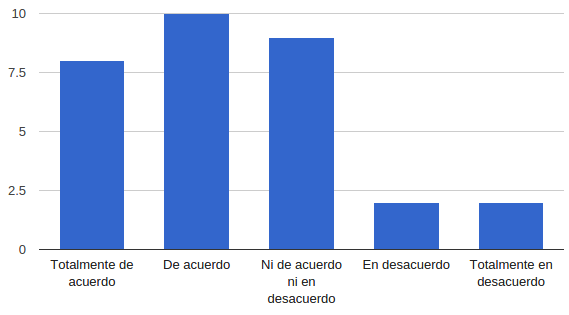
\includegraphics[scale=0.5]{C_DSL_reutilizable.png}
  \end{center}
  \caption{Resumen de votos para la característica de la capacidad de reutilización}
  \label{fig:evalmetodo:dsl:reutilizable}
\end{figure}

Hay una mayoría de docentes que están en mayor o menor medida de acuerdo con la consecución de esta característica (18 de 31). Además, 9 docentes mostraron una posición neutral con respecto a esta característica, mientras que 4 estuvieron en desacuerdo. Los docentes que estuvieron en desacuerdo fueron nuevamente docentes de Ciencias o Ciencias de la salud.

\begin{figure}[h]
  \begin{center}
    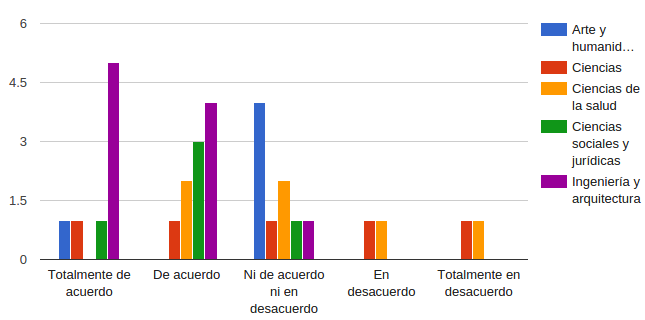
\includegraphics[scale=0.5]{C_DSL_reutilizable_rama.png}
  \end{center}
  \caption{Resumen de votos para la característica de la capacidad de reutilización por rama}
  \label{fig:evalmetodo:dsl:reutilizable:rama}
\end{figure}

\newpage
\paragraph*{Fiabilidad}

El resumen de respuestas para la característica de la fiabilidad del DSL puede verse en las figuras~\ref{fig:evalmetodo:dsl:fiabilidad} y~\ref{fig:evalmetodo:dsl:fiabilidad:rama}.

\begin{figure}[h]
  \begin{center}
    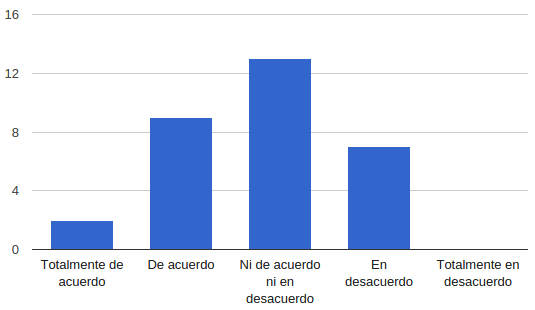
\includegraphics[scale=0.5]{C_DSL_fiabilidad.png}
  \end{center}
  \caption{Resumen de votos para la característica de la fiabilidad}
  \label{fig:evalmetodo:dsl:fiabilidad}
\end{figure}

Hay una mayoría de docentes que están en una posición neutra (13 de 31). Además, 11 docentes mostraron estar en mayor o menor medida de acuerdo con respecto a esta característica, mientras que 7 estuvieron en desacuerdo. 

\begin{figure}[h]
  \begin{center}
    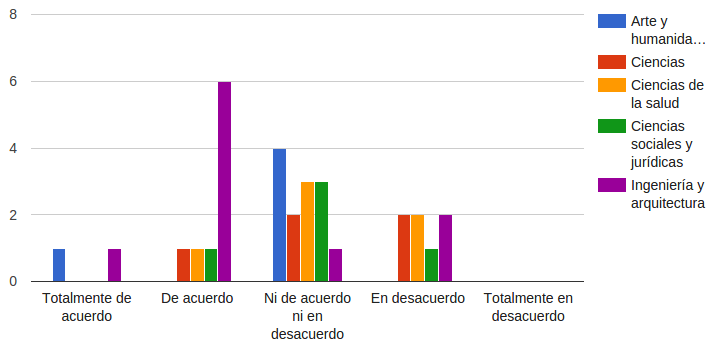
\includegraphics[scale=0.5]{C_DSL_fiabilidad_rama.png}
  \end{center}
  \caption{Resumen de votos para la característica de la fiabilidad por rama}
  \label{fig:evalmetodo:dsl:fiabilidad:rama}
\end{figure}
    

%-----------------------------------------------------------------
%-----------------------------------------------------------------
%-----------------------------------------------------------------
\subsection{Evaluación de la sintaxis del DSL (consulta tipo)}

Con respecto a la pregunta sobre la entendibilidad de la sintaxis del DSL, el resumen de las respuestas puede verse en la tabla~\ref{tab:evalmetodo:encuesta:metodoDBA:rama}.

\begin{table}[H]
  \begin{center}
  \begin{tabular}{| l | l | r | r | r |}
    \hline
    & Rama & Sí & No & Total \\
    \hline
    \hline
    \multirow{2}{2.5cm}{SSH} & Arte y humanidades & 2 & 3 & 5  \\
    \cline{2-5}
    & Ciencias sociales y jurídicas & 3 & 2 & 5  \\
    \hline
    \multirow{3}{2.5cm}{EHSE} & Ciencias & 5 & 0 & 5  \\
    \cline{2-5}
    & Ciencias de la salud & 5 & 1 & 6  \\
    \cline{2-5}
    & Ingeniería y arquitectura & 9 & 1 & 10 \\
    \hline
  \end{tabular}
\end{center}
\caption{Consideración de la consulta como entendible o no por ramas}
\label{tab:evalmetodo:encuesta:consulta:rama}
\end{table}

Un 77\percentage{ }de los encuestados (24 de 31) consideraron la sintaxis DSL entendible. Para dar validez a los resultados es necesario determinar la independencia de los mismos.

En primer lugar, para determinar si existe relación entre la respuesta de cada docente y su rama se define la siguiente hipótesis nula:

\medskip
\begin{mdframed}[style=hipotesis0]
$H_0$: \emph{La consideración por parte de un docente de que la sintaxis del DSL sea o no entendible es independiente de la rama de dicho docente}
\end{mdframed}

\medskip
Para contrastar la hipótesis se utilizó el test exacto de Fisher, no pudiéndose rechazar la hipótesis con un \textbf{p-valor de 0,121}, superior al umbral de significación del 0,005. Por lo que se concluye que, con una significación del 5\percentage, los datos son independientes.

En segundo lugar, para determinar si existe relación entre la respuesta de cada docente y su rama principal se define la siguiente hipótesis nula:

\medskip
\begin{mdframed}[style=hipotesis0]
$H_0$: \emph{La consideración por parte de un docente de que la sintaxis del DSL sea o no entendible es independiente de si dicho docente es de EHSE o de SSH}
\end{mdframed}

\medskip
Para contrastar la hipótesis se utilizó el test exacto de Fisher, no pudiéndose rechazar la hipótesis con un \textbf{p-valor de 0,021}, superior al umbral de significación del 0,005. Por lo que se concluye que, con una significación del 5\percentage, los datos son independientes.

%-----------------------------------------------------------------
%-----------------------------------------------------------------
%-----------------------------------------------------------------
\subsection{Evaluación de los resultados}

Con respecto a la pregunta sobre la entendibilidad de los resultados devueltos por el DSL, el resumen de las respuestas puede verse en la tabla~\ref{tab:evalmetodo:encuesta:metodoDBA:rama}.

\begin{table}[H]
  \begin{center}
  \begin{tabular}{| l | l | r | r | r |}
    \hline
    & Rama & Sí & No & Total \\
    \hline
    \hline
    \multirow{2}{2.5cm}{SSH} & Arte y humanidades & 3 & 2 & 5  \\
    \cline{2-5}
    & Ciencias sociales y jurídicas & 0 & 5 & 5  \\
    \hline
    \multirow{3}{2.5cm}{EHSE} & Ciencias & 5 & 0 & 5  \\
    \cline{2-5}
    & Ciencias de la salud & 5 & 1 & 6  \\
    \cline{2-5}
    & Ingeniería y arquitectura & 7 & 3 & 10 \\
    \hline
  \end{tabular}
\end{center}
\caption{Consideración de los resultados como entendibles o no por ramas}
\label{tab:evalmetodo:encuesta:resultados:rama}
\end{table}

Un 64\percentage{ }de los encuestados (20 de 31) consideraron los resultados entendibles. Para dar validez a los resultados del cuestionario es necesario determinar la independencia de los mismos.

En primer lugar, para determinar si existe relación entre la respuesta de cada docente y su rama se define la siguiente hipótesis nula:

\medskip
\begin{mdframed}[style=hipotesis0]
$H_0$: \emph{La consideración por parte de un docente de que los resultados sean o no entendibles es independiente de la rama de dicho docente}
\end{mdframed}

\medskip
Para contrastar la hipótesis se utilizó el test exacto de Fisher, no pudiéndose rechazar la hipótesis con un \textbf{p-valor de 0,010}, superior al umbral de significación del 0,005. Por lo que se concluye que, con una significación del 5\percentage, los datos son independientes.

En segundo lugar, para determinar si existe relación entre la respuesta de cada docente y su rama principa se define la siguiente hipótesis nula:

\medskip
\begin{mdframed}[style=hipotesis0]
$H_0$: \emph{La consideración por parte de un docente de que los resultados sean o no entendibles es independiente de si dicho docente es de EHSE o de SSH}
\end{mdframed}

\medskip
Para contrastar la hipótesis se utilizó el test exacto de Fisher, no pudiéndose rechazar la hipótesis con un \textbf{p-valor de 0,013}, superior al umbral de significación del 0,005. Por lo que se concluye que, con una significación del 5\percentage, los datos son independientes.
